%label:"con:symplecticCohomologyQuadratic"
%author:JeffHicks
%name:"$\SH(X)$ via quadratic $H$"
%type:"construction"


   \label{con:symplecticCohomologyQuadratic}
   Let $(X, \lambda)$ be a Liouville domain, and let $\hat X$ be its completion. The goal is to construct a Floer cohomology which witnesses all of the Reeb orbits of $\partial X$. With that in mind, it is natural to study the Hamiltonian Floer cohomology of Hamiltonians $H_t$ with the property that over the symplectization they are of the form 
   \[H|_{\RR\times \partial X}=h(\exp(r))\]
   where $\lim_{r\to\infty} h'(\exp(r))=\infty$. This Hamiltonian witnesses every Reeb orbit with sufficiently large period. 
   %label:"fig:quadraticHamiltonian"
%author:JeffHicks
%name:"quadratic Hamiltonian"
%type:"figure"
%parent:con:symplecticCohomologyQuadratic
%caption:"An increasing Hamiltonian over the symplectization witnesses all Reeb orbits"


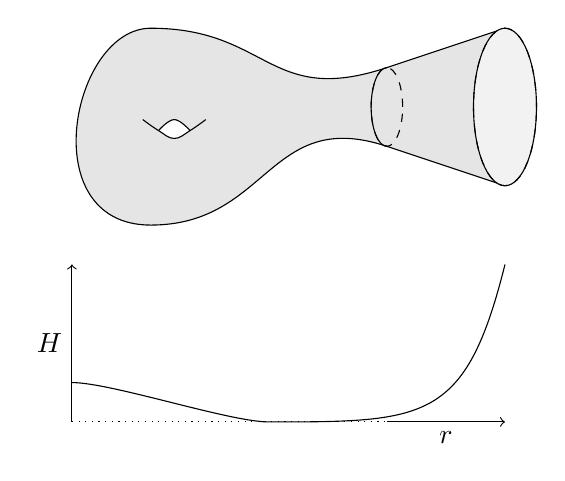
\begin{tikzpicture}
    \draw[fill=gray!20] (4,-0.5) .. controls (2.5,-1) and (4,-0.5) .. (2.5,-1) .. controls (1,-1.5) and (1,-0.5) .. (-0.5,-0.5) .. controls (-1.5,-0.5) and (-2,-3) .. (-0.5,-3) .. controls (1,-3) and (1,-1.5) .. (2.5,-2) .. controls (4,-2.5) and (2.5,-2) .. (4,-2.5);
    \begin{scope}[shift={(3.2,-2)}]
    
    \fill[white]  plot[smooth, tension=0.7] coordinates { (-3.6,0.2) (-3.4,0.1) (-3.2,0.2) }  plot[smooth, tension=0.7] coordinates {(-3.6,0.2) (-3.4,0.34) (-3.2,0.2)};
    
    \draw  plot[smooth, tension=0.7] coordinates {(-3.8,0.34) (-3.6,0.2) (-3.4,0.1) (-3.2,0.2) (-3,0.34)};
    \draw  plot[smooth, tension=0.7] coordinates {(-3.6,0.2) (-3.4,0.34) (-3.2,0.2)};
    
    
    
    \end{scope}
    
    \begin{scope}[]
    
    \draw[dashed]  (2.5,-1.5) ellipse (0.2 and 0.5);
    \clip  (2,-1) rectangle (2.5,-2);
    
    \draw  (2.5,-1.5) ellipse (0.2 and 0.5);
    \end{scope}
    
    \begin{scope}[scale=2, shift={(-0.5,0.75)}]
    
    \draw[dashed, fill=gray!10]  (2.5,-1.5) ellipse (0.2 and 0.5);
    
    
    \draw  (2.5,-1.5) ellipse (0.2 and 0.5);
    \end{scope}
    
    \draw[dotted] (-1.5,-5.5) -- (2.5,-5.5);
    \draw[->] (2.5,-5.5) --node[below]{$r$} (4,-5.5);
    \draw (-1.5,-5) .. controls (-1,-5) and (0.5,-5.5) .. (1,-5.5) .. controls (3,-5.5) and (3.5,-5.5) .. (4,-3.5);
    
    \draw[->] (-1.5,-5.5) -- node[left]{$H$} (-1.5,-3.5);
    \end{tikzpicture}
   
   A problem with this definition is that the Hamiltonian we have chosen is time independent, and so whenever $(\partial X, \alpha)$ has any Reeb orbits, the time-1 orbits of $H$ will necessarily be degenerate (all orbits come in $S^1$ families from reparameterization). The standard work-around is to introduce a small time-dependent perturbation to $H$ in such a way that we can still apply our maximum principle argument. We therefore look at time-dependent Hamiltonians $H_t$ which, outside of a compact set, are of the form $h_t(\exp(r))$, with $\lim_{r\to\infty} h_t(\exp(r))=\infty$ for all $t$. The maximum principle argument from \cref{prp:liouvilleIsGeometricallyBounded} can be made to hold in this setting (Proposition 4.1 \cite{wendlbeginner}).

   One then takes the definition of the symplectic cohomology to be 
   \[\SH(X):=\CF(\hat X, H_t)=\bigoplus_{\gamma\st \dot \gamma= V_{H_t}} \ZZ\langle \gamma\rangle.\]
   with differential given by structure coefficients $\langle d(\gamma_+), \gamma_\rangle$ counting $V_{H_t}$-perturbed pseudoholomorphic cylinders with ends limiting to $\gamma_\pm$.
